%-------------------------------------------------------------------------------
\section{Einführung in das Semester}
%-------------------------------------------------------------------------------

%%% Folie
\begin{frame}{Kompetenzziele der Vorlesung}
    \begin{itemize}
        \item \textbf{Fachkompetenz:} Die Studierenden kennen den technischen Aufbau typischer
        Devices/Embedded Systems im Kontext der Internet of Things. Sie sind in der Lage,
        entsprechende Devices für einen gegebenen Einsatzzweck auszuwählen und zu programmieren.
        \medskip

        \item \textbf{Methodenkompetenz:} Die Studierenden sind in der Lage bei der Programmierung
        von IoT-Geräten systematisch und methodisch vorzugehen.
        \medskip

        \item \textbf{Personale und soziale Kompetenz:} Die Studierenden verstehen die Herausforderungen
        des IoT für Unternehmen, Politik und Gesellschaft und sind in der Lage, diese kompetent zu diskutieren.
        \medskip

        \item \textbf{Übergreifende Handlungskompetenz:} Die Studierenden können reale betriebliche
        Problemstellungen im Kontext von IoT analysieren, Konzepte entwerfen und IoT-fähige Geräte
        programmieren und im Unternehmenskontext integrieren.
        \medskip
    \end{itemize}
\end{frame}

{
\footnotesize
%%% Folie
\begin{frame}{Inhalte der Vorlesung}
        \begin{columns}
            \begin{column}[T]{.5\textwidth}
                \begin{block}{3. Semester}
                    \medskip
                    \textbf{Prüfungsform:} Klausur
                    \medskip

                    \begin{enumerate}
                        \item Grundlagen des Internet of Things
                        \item Hardwaredesign für IoT-Anwendungen
                        \item \textcolor{gray}{Übungsstunde}
                        \item \textcolor{gray}{Übungsstunde}
                        \item Einführung in Python
                        \item IoT-Entwicklung mit Python
                        \item \textcolor{gray}{Übungsstunde}
                        \item \textcolor{gray}{Übungsstunde}
                        \item \textcolor{gray}{Klausurvorbereitung}
                    \end{enumerate}
                \end{block}
            \end{column}
            \begin{column}[T]{.5\textwidth}
                \begin{block}{4. Semester}
                    \medskip
                    \textbf{Prüfungsform:} Assignment
                    \medskip

                    \begin{enumerate}
                        \item Nutzung analoger und digitaler Bauteile
                        \item Python-Architekturmuster für IoT-Devices
                        \item Datenaustausch und Systemintegration
                        \item Linux-Konfiguration und Deployment
                        \item \textcolor{gray}{Assignment}
                        \item \textcolor{gray}{Assignment}
                        \item \textcolor{gray}{Assignment}
                        \item \textcolor{gray}{Assignment}
                        \item \textcolor{gray}{Assignment}
                    \end{enumerate}
                \end{block}
            \end{column}
        \end{columns}
\end{frame}
}

%%% Folie
{
\setbeamertemplate{background canvas}{
    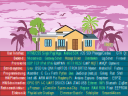
\includegraphics[height=\paperheight, width=\paperwidth]{1-grundlagen/img/themengebiete4}
}

\begin{frame}[plain]
\end{frame}
}

%%% Folie
\begin{frame}{Beispiel einer typischen IoT-Architektur}
    \begin{columns}
        \column{\dimexpr\paperwidth-10pt}
        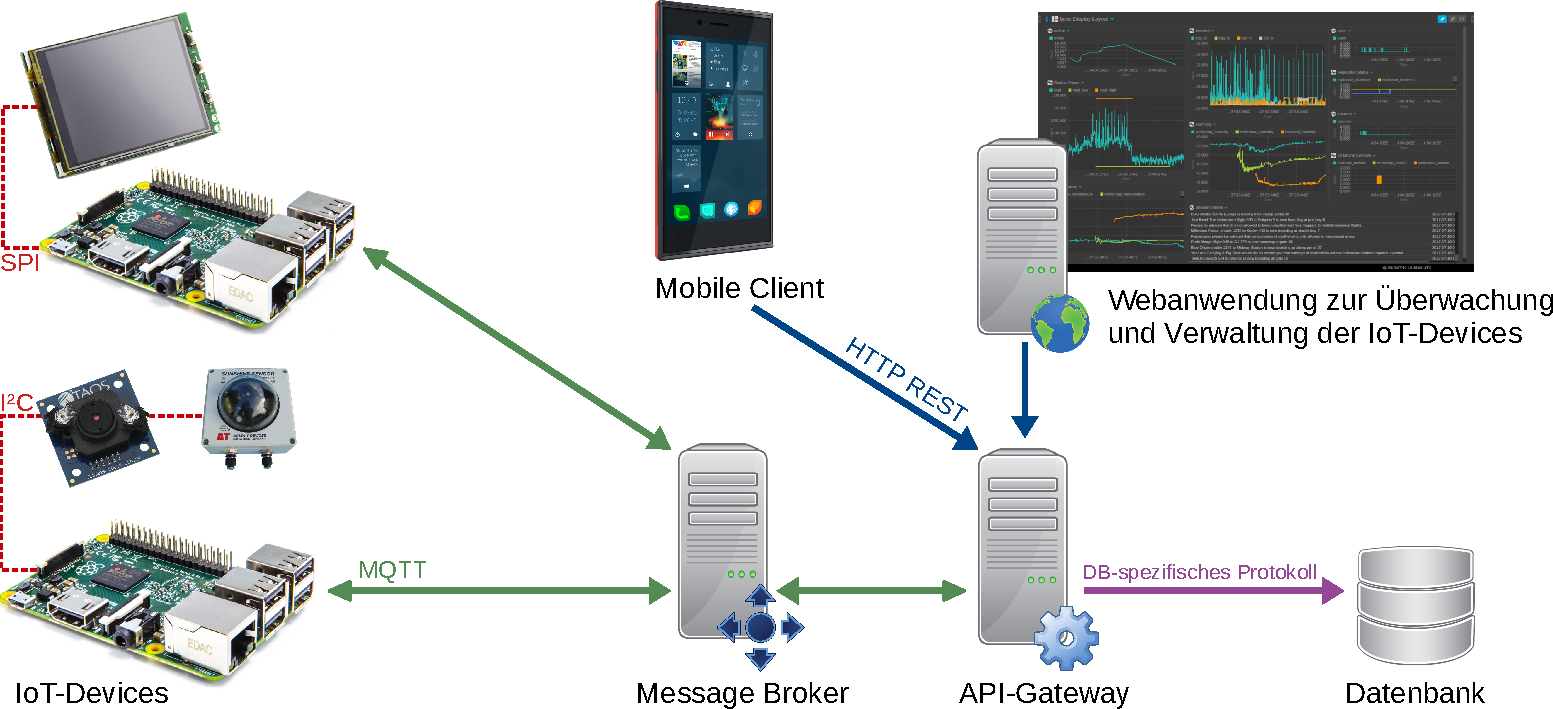
\includegraphics[width=\textwidth]{1-grundlagen/img/architektur_beispiel}
    \end{columns}
\end{frame}

%%% Folie
{
\small

\begin{frame}{Inhalt der Assignment-Prüfung}
    \begin{columns}[onlytextwidth]
        \column[t]{.45\textwidth}
        \begin{block}{Kreativaufgabe}
            \medskip
            \parbox{\linewidth}{
                Ausarbeitung eines Hard- und Softwareentwurfs zu einem \textbf{selbst gewählten IoT-Anwendungsfall}.
                \medskip

                Muss die wesentlichen Theorieinhalte beider Semester abdecken.
                \medskip

                Jedoch keinen Quellcode, keine Details und keine praktische Umsetzung. Nur das Konzept.
            }
        \end{block}

        \column[t]{.45\textwidth}
        \begin{block}{Programmieraufgabe}
            \medskip
            \parbox{\linewidth}{
                Praktische Umsetzung eines \textbf{vorgegebenen IoT-Anwendungsfalls}.
                \medskip

                Muss gegen vorgegebene Schnittstellen zum Mocken der Hardwareelemente
                programmiert werden.
                \medskip

                Bewertet werden die Qualität des Quellcodes und die Erfüllung der von
                uns vorgegebenen Unit Tests.
            }
        \end{block}
    \end{columns}

    \bigskip
    \bigskip
    {
        \normalsize
        Die Aufgabenstellung wird bis zum Ende des Theorieblocks bereitgestellt.
    }
\end{frame}
}

%%% Folie
{
\small
\setlength{\fboxsep}{0pt}

\begin{frame}{Literaturempfehlungen}
    \begin{columns}
        \column[b]{.25\textwidth}
        \fbox{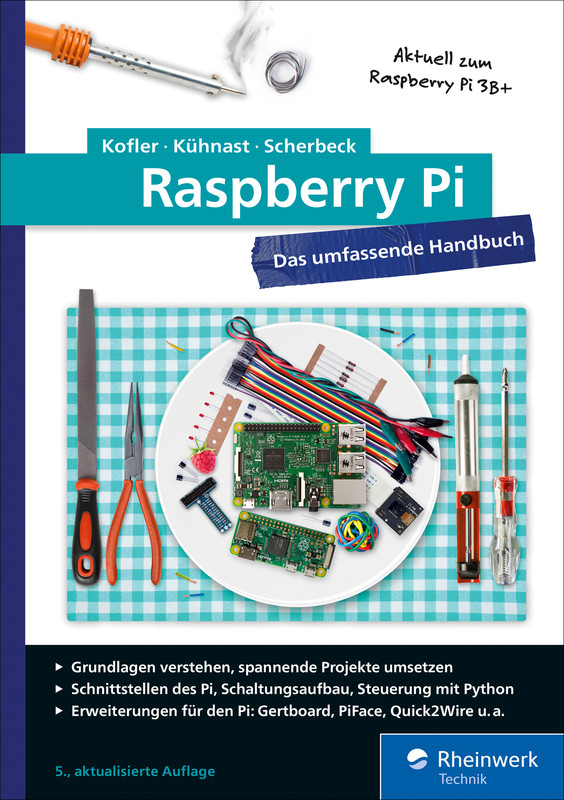
\includegraphics[height=3.8cm]{5-hardwarenutzung/img/buch_raspberrypi}}

        \column[b]{.25\textwidth}
        \fbox{
\includegraphics[height=3.8cm]{5-hardwarenutzung/img/buch_mqtt_essentials}}

        \column[b]{.25\textwidth}
        \fbox{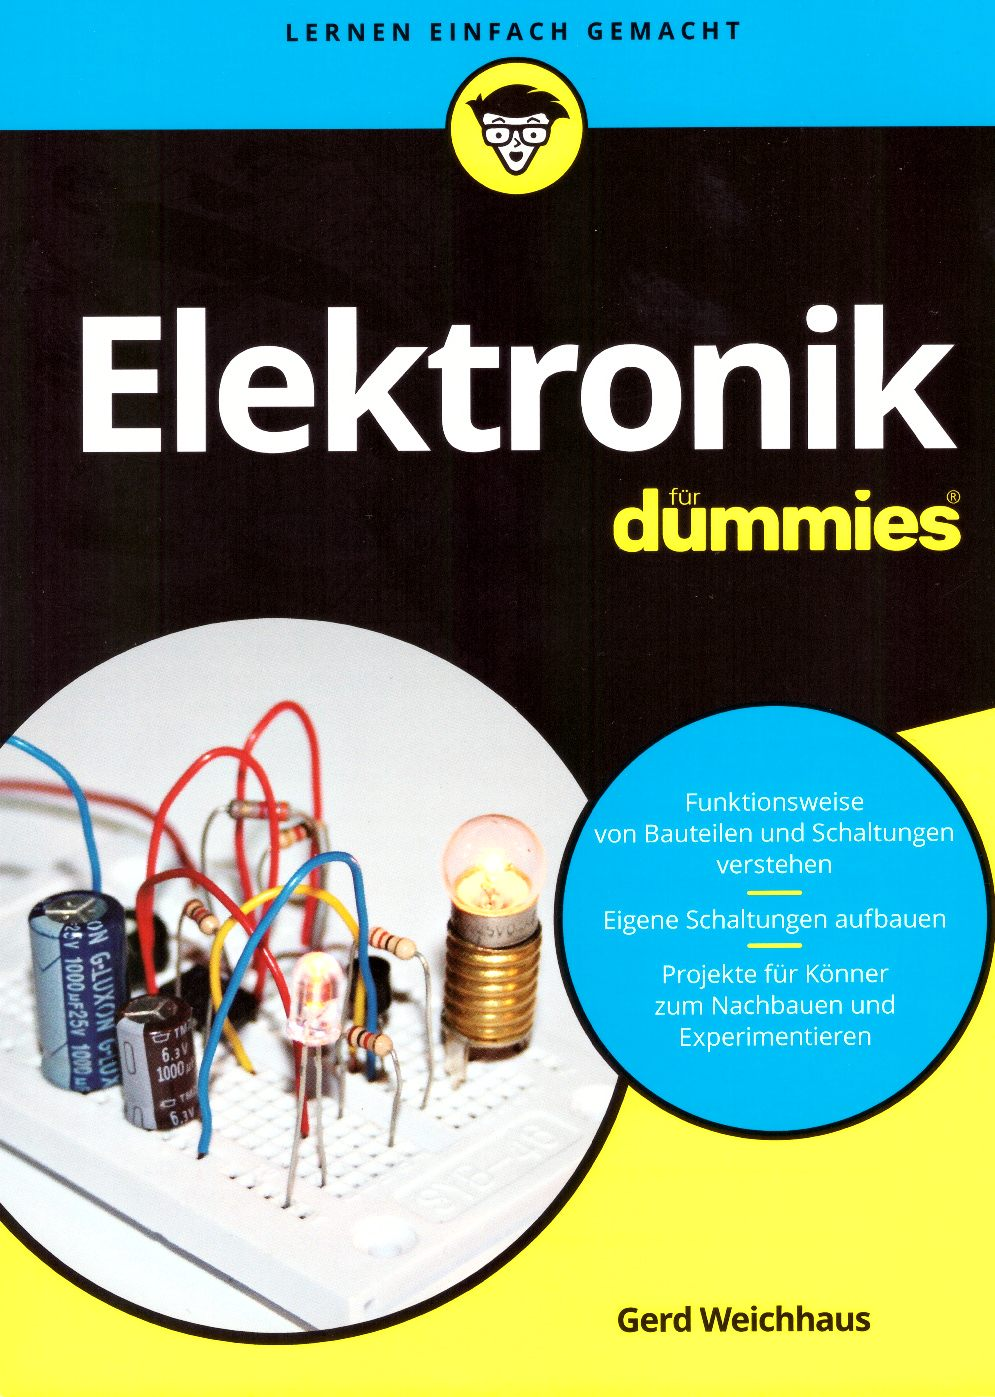
\includegraphics[height=3.8cm]{5-hardwarenutzung/img/buch_elektronik_dummies}}

        \column[b]{.25\textwidth}
        \fbox{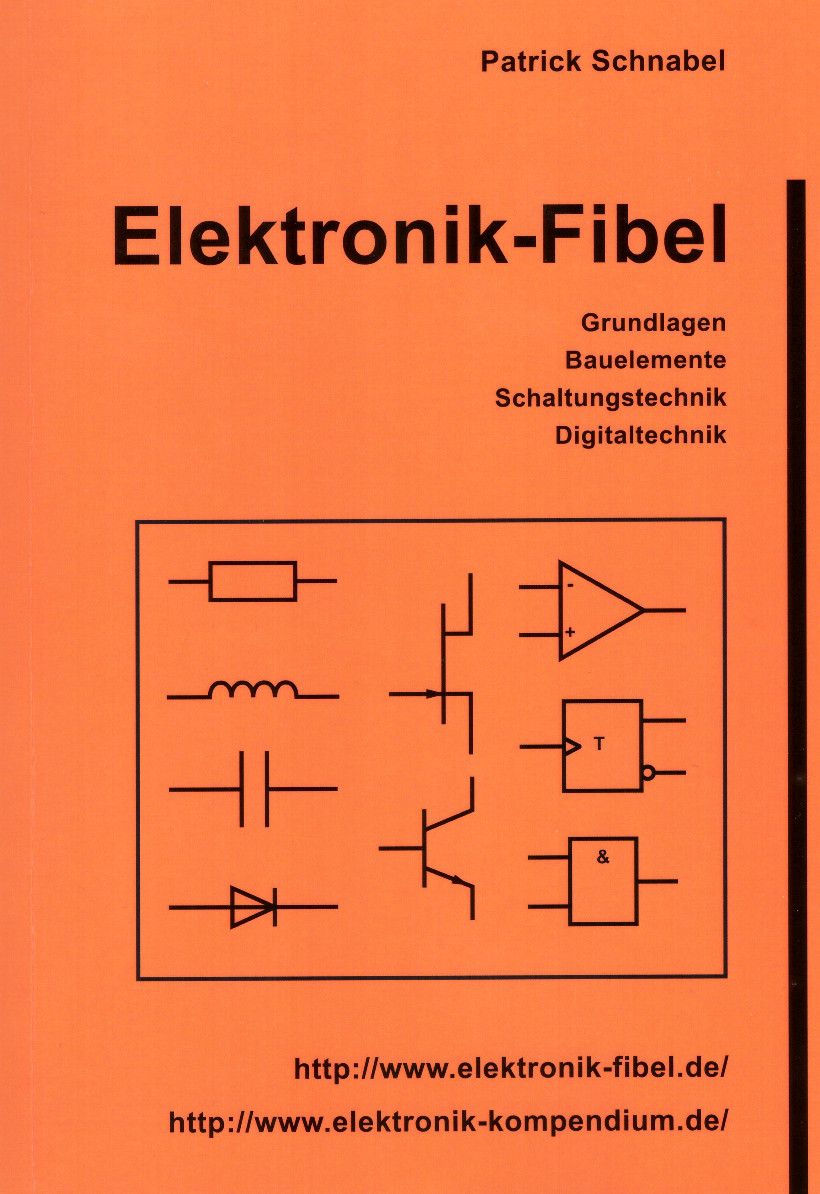
\includegraphics[height=3.8cm]{5-hardwarenutzung/img/buch_elektronik_fibel}}
    \end{columns}

    \vskip 0.6cm

    \begin{columns}
        \column[T]{.5\textwidth}
        \textbf{Raspberry Pi: Das umfassende Handbuch für Maker und Tekkies} \\ Rheinwerk Verlag, 2018

        \column[T]{.5\textwidth}
        \textbf{MQTT Essentials: \\ A Lightweight IoT Protocol} \\ Packt>, 2017
    \end{columns}

    \vskip 0.6cm

    \begin{columns}
        \column[T]{.5\textwidth}
        \textbf{Elektronik für Dummies} \\ Wiley-VCH Verlag, 2018

        \column[T]{.5\textwidth}
        \textbf{Elektronik-Fibel} \\ Patrick Schnabel, 2017
    \end{columns}
\end{frame}
}

%-------------------------------------------------------------------------------
\section{Ziel der heutigen Vorlesung}
%-------------------------------------------------------------------------------

%%% Folie
{
\footnotesize
\setlength{\leftmargini}{1.2em}

\begin{frame}{Typischer Systemaufbau eingebetteter Systeme}
    \begin{columns}
        \column{\dimexpr\paperwidth}

        \only<beamer:1|handout:0>{
            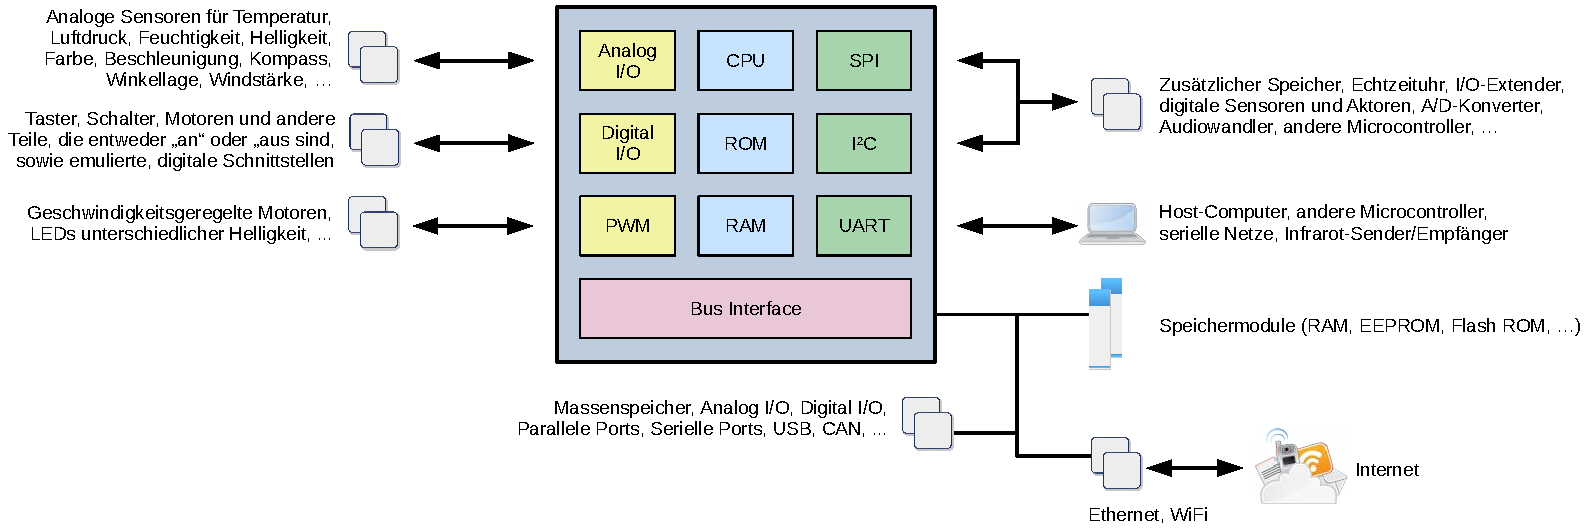
\includegraphics[width=\paperwidth]{5-hardwarenutzung/img/mc_aufbau1}
        }

        \only<beamer:2|handout:1>{
            \transdissolve
            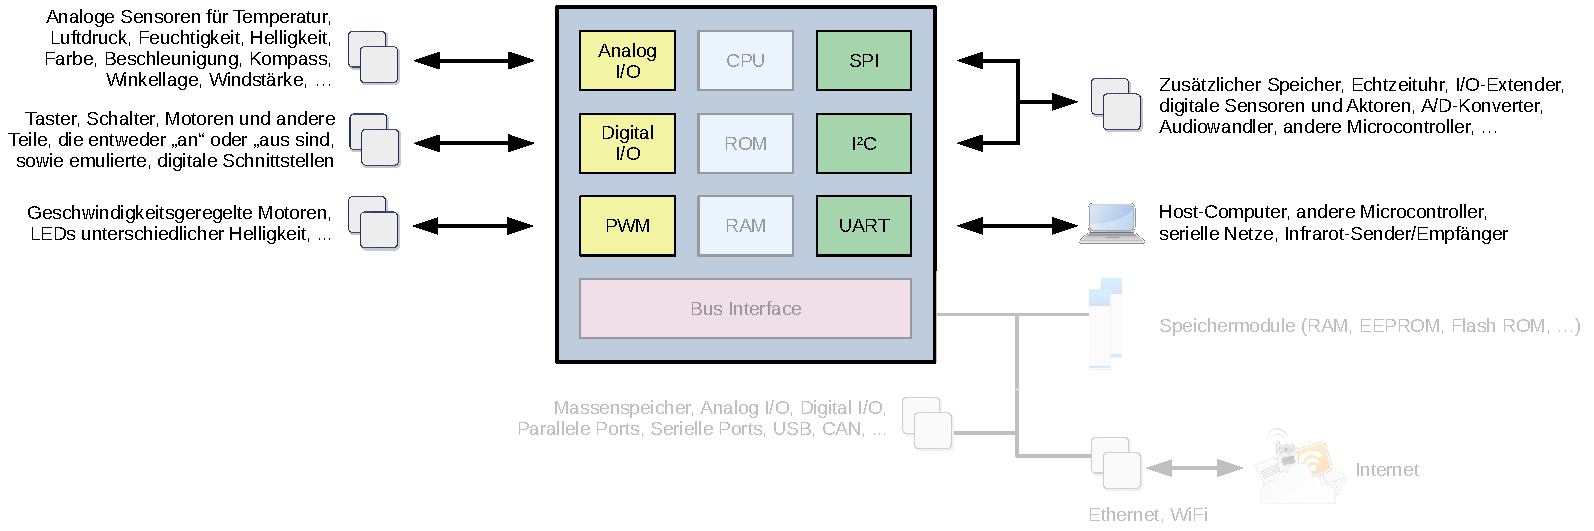
\includegraphics[width=\paperwidth]{5-hardwarenutzung/img/mc_aufbau2}
        }
    \end{columns}

    \medskip

    \begin{columns}
        \begin{column}[T]{.3\textwidth}
            \textbf{Raspberry Pi}
            \begin{itemize}
                \item Binäre Ein-/Ausgänge
                \item PWM-Ausgänge
                \item Serielle Ein-/Ausgänge
                \item<2> \textcolor{darkred}{Kein Analog I/O}
                \item<2> \textcolor{darkred}{Keine Bus Interface!}
            \end{itemize}
        \end{column}
        \begin{column}[T]{.3\textwidth}
            \textbf{Letztes Semester}
            \begin{itemize}
                \item Binäre Ein-/Ausgänge
                \item PWM-Ausgänge
                \item DHT11 via 1-Wire
                \item Programmierung in Python
            \end{itemize}
        \end{column}
        \begin{column}[T]{.3\textwidth}
            \textbf{Dieses Semester}
            \begin{itemize}
                \item Analog-Digital-Konverter
                \item Serielle Sensoren/Aktoren
                \item Serielle Kommunikation mit anderen µControllern
                \item Programmierung in Python
            \end{itemize}
        \end{column}
    \end{columns}
\end{frame}
}

%%% Folie
{
\scriptsize

\begin{frame}{Inhalt unseres Sensorkits}
    \begin{columns}
        \column[T]{.3\textwidth}
        \textbf{Analoge Schnittstelle} \\
        KY-003: Hall Magnetfeldsensor \\
        KY-006: Passiver Piezo-Buzzer \\
        KY-009: RGB-LED \\
        KY-011: Rot/Grün-LED \\
        KY-012: Aktiver Piezo-Buzzer \\
        KY-013: Temperatursensor \\
        KY-016: RGB-LED \\
        KY-018: Fotowiderstand \\
        KY-023: XY-Joystick \\
        KY-024: Magnetic Hall-Sensor \\
        KY-025: Reedkontakt \\
        KY-026: Flammensensor \\
        KY-028: Thermistor \\
        KY-029: Rot/Grün-LED \\
        KY-034: 7-Farben LED \\
        KY-035: Bihor Magnetsensor \\
        KY-036: Metall-Touchsensor \\
        KY-037: Mikrofon Soundsensor \\
        KY-038: Mikrofon Soundsensor \\
        KY-039: Herzschlagsensor \\
        KY-040: Kodierter Drehschalter \\
        KY-050: Ultraschallabstand \\

        \column[T]{.3\textwidth}
        \textbf{Binäre An/Aus-Schnittstelle} \\
        KY-002: Erschütterungsschalter \\
        KY-003: Hall Magnetfeldsensor \\
        KY-004: Taster \\
        KY-010: Lichtschranke \\
        KY-012: Aktiver Piezo-Buzzer \\
        KY-017: Neigungsschalter \\
        KY-019: 5V Relais \\
        KY-020: Neigungsschalter \\
        KY-021: Mini Magnet-Reedkontakt \\
        KY-024: Magnetic Hall-Sensor \\
        KY-025: Reedkontakt \\
        KY-026: Flammensensor \\
        KY-027: Magic Light Cup \\
        KY-028: Thermistor \\
        KY-031: Klopfsensor \\
        KY-032: Hindernisdetektor \\
        KY-033: Trackingsensor \\
        KY-036: Metall-Touchsensor \\
        KY-037: Mikrofon Soundsensor \\
        KY-038: Mikrofon Soundsensor \\

        \column[T]{.3\textwidth}
        \textbf{Serielle Schnittstelle} \\
        KY-001: DS18B20 Temperatur \\
        KY-015: DHT11 Temp./Feuchtig. \\
        KY-052: BMP280 Druck \\
        KY-053: Analog/Digital Konverter \\
    \end{columns}
\end{frame}
}

%%% Folie
\begin{frame}{Lernziele}
    \begin{block}{Wiederholung}
        \begin{itemize}
            \item Binäre Bauteile via GPIO mit dem Pi verbinden können
            \item Via GPIO angebundene Bauteile in Python nutzen können
            \item Breadboards zum Aufbau einfacher Schaltungen nutzen können
        \end{itemize}
    \end{block}

    \begin{block}{Neue Inhalte}
        \begin{itemize}
            \item Funktionsweise serieller Schnittstellen erklären können
            \item Synchrone und asynchrone, serielle Schnittstellen abgrenzen können
            \item Digitale Bauteile via SPI, I²C mit dem Pi verbinden können
            \item Analoge Bauteile via A/D-Konverter mit dem Pi verbinden können
            \item Seriell angebundene Bauteile in Python nutzen können
        \end{itemize}
    \end{block}
\end{frame}

%-------------------------------------------------------------------------------
\section{Nutzung binärer Bauteile}
%-------------------------------------------------------------------------------

% PWM-Folie übernehmen / anpassen
% Fallbeispiele wie in die Folien/Vorlesung integrieren?
% Wie viel Quellcode in den Folien zeigen?
% Auf jeden Fall erst die Theorie, dann die Programmierung je Kapitel

%%% Folie
\begin{frame}{Folie}
    TODO
\end{frame}

%%% Folie
\begin{frame}{Folie}
    TODO
\end{frame}

%-------------------------------------------------------------------------------
\section{Serielle Kommunikation}
%-------------------------------------------------------------------------------

% Folie mit den Einsatzgebieten übernehmen / anpassen
% Folie mit der Übersichtsgrafik übernehmen / anpassen

%%% Folie
\begin{frame}{Folie}
    TODO
\end{frame}

%%% Folie
\begin{frame}{Folie}
    TODO
\end{frame}
